
\section{Experimentations}

\begin{figure*}
  \centering
  \subfloat[Référentiel Logoot]
  [\label{fig:logoot}Logoot comme stratégie d'allocation référentielle.]
  {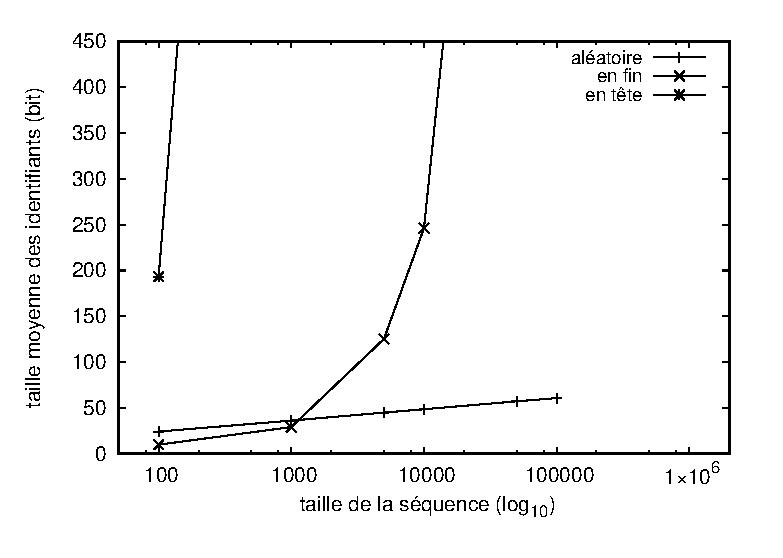
\includegraphics[width=0.48\textwidth]{./img/lseq/logoot.eps}}
  \hspace{10pt}
  \subfloat[Alternance de stratégies]
  [\label{fig:robin}Alternance de stratégie d'allocation antagonistes.]
  {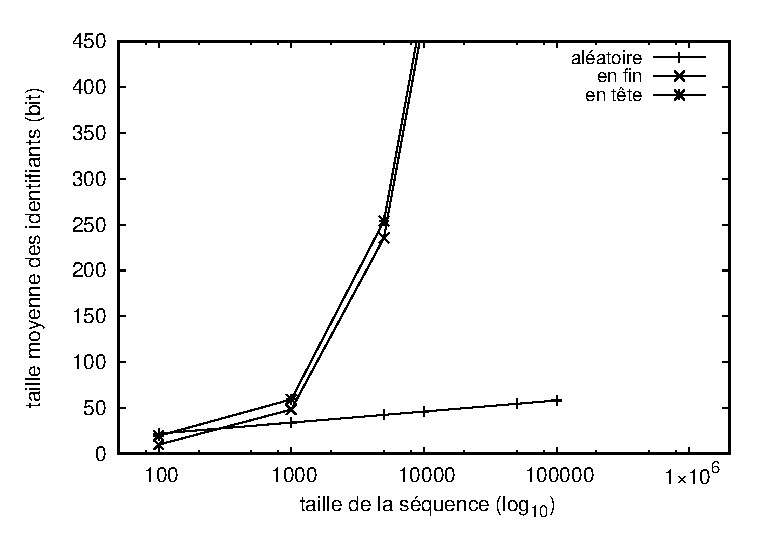
\includegraphics[width=0.48\textwidth]{./img/lseq/robin.eps}}
\end{figure*}

\begin{figure*}
  \centering
  \subfloat[Augmentation de l'espace d'allocation]
  [\label{fig:double}Augmentation de l'espace d'allocation en fonction de 
  la profondeur de l'arbre.]
  {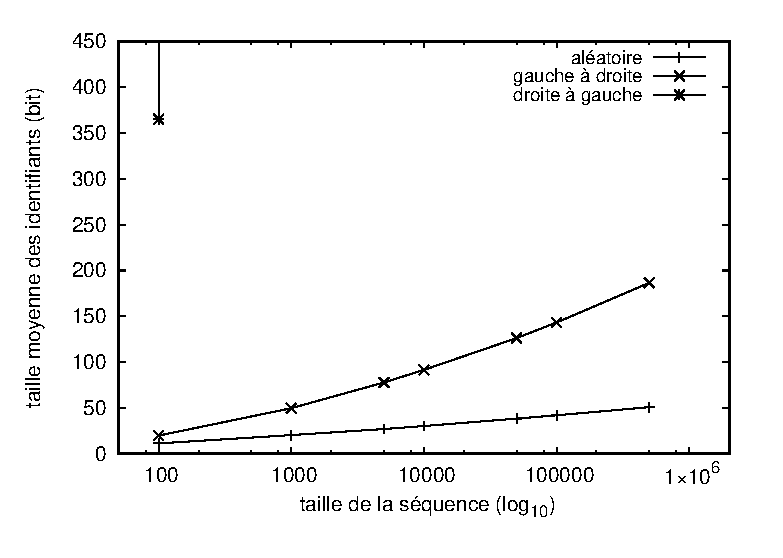
\includegraphics[width=0.48\textwidth]{./img/lseq/double.eps}}
  \hspace{10pt}
  \subfloat[Alternance et augmentation de l'espace d'allocation]
  [\label{fig:lseq}\LSEQ comme combinaison de l'alternance et de l'augmentation.]
  {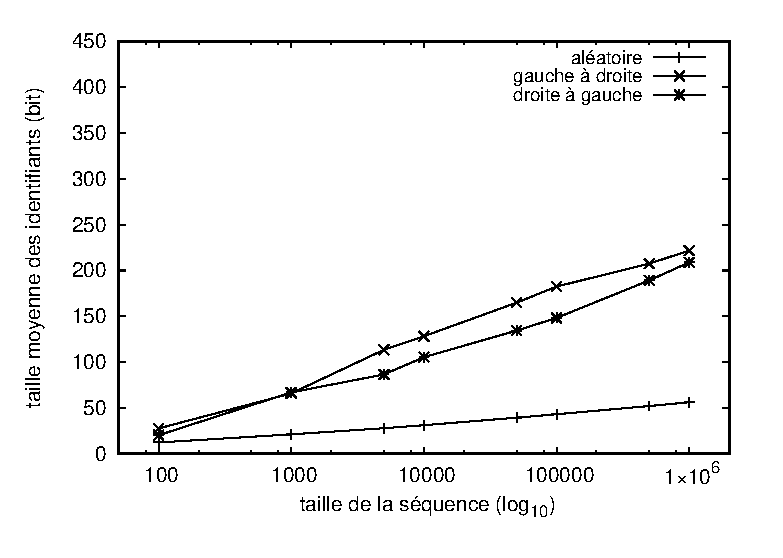
\includegraphics[width=0.48\textwidth]{./img/lseq/lseq.eps}}
\end{figure*}


\begin{figure*}
  \centering
  \subfloat[Utilisateur unique]
  [\label{fig:one}Augmentation de l'espace d'allocation en fonction de 
  la profondeur de l'arbre.]
  {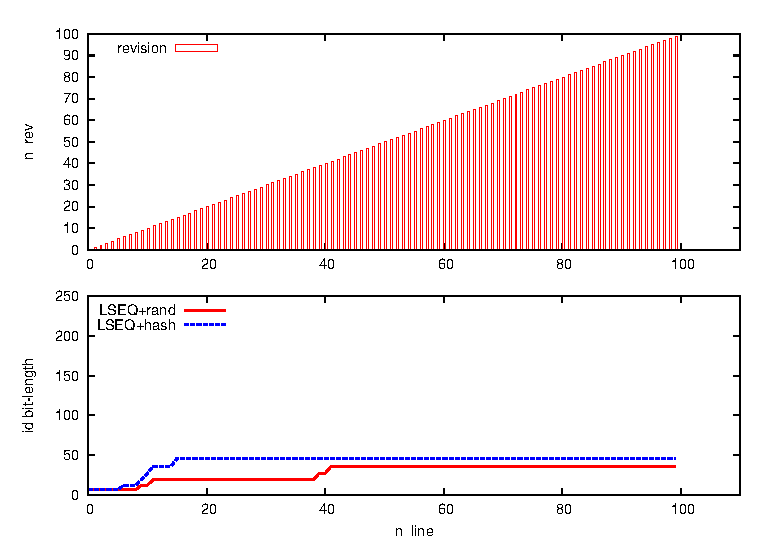
\includegraphics[width=0.48\textwidth]{./img/lseq/oneuser.eps}}
  \hspace{10pt}
  \subfloat[Alternance et augmentation de l'espace d'allocation]
  [\label{fig:ten}\LSEQ comme combinaison de l'alternance et de l'augmentation.]
  {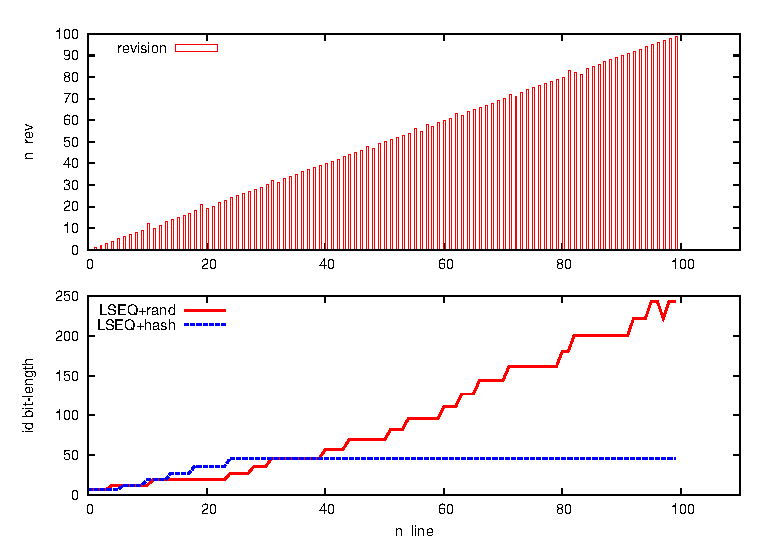
\includegraphics[width=0.48\textwidth]{./img/lseq/tenusers.eps}}
  \caption{Spectre de document artificiel générés par insertion répétée de caractère
  en queue.}
\end{figure*}



\begin{figure*}
  \centering
  \subfloat[Comportement d'édition attendu]
  [\label{fig:compliant}Le comportement d'édition correspond aux attentes
  de la stratégie d'allocation]
  {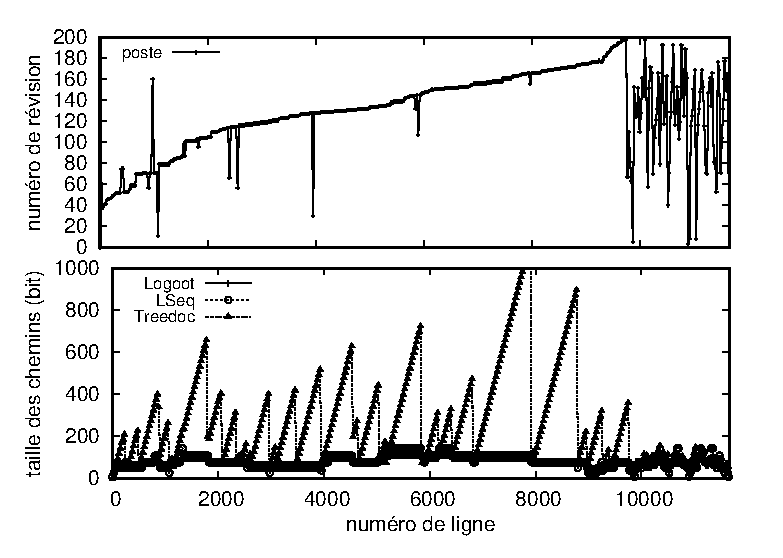
\includegraphics[width=0.48\textwidth]{./img/lseq/poste.eps}}
  \hspace{10pt}
  \subfloat[Comportement d'édition inattendu]
  [\label{fig:motivating}Le comportement d'édition va à l'encontre des attentes
  de la stratégie d'allocation]
  {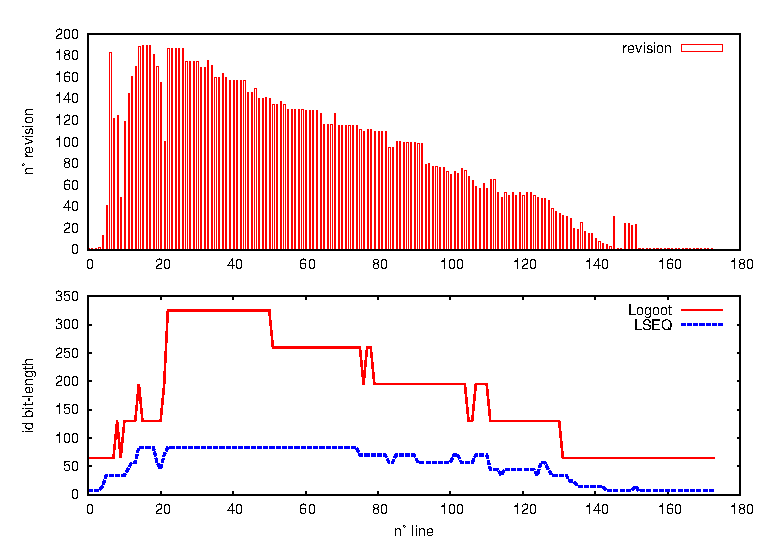
\includegraphics[width=0.48\textwidth]{./img/lseq/didyouknow.eps}}
  \caption{\label{fig:allocation}Spectre de document Wikipedia sous différent
    comportements d'édition antagonistes. La figure du haut représente la
    révision à laquelle la ligne a été inséré, i.e., sa date de naissance.  La
    figure du bas représente la taille de l'identifiant associé à chaque ligne.}
\end{figure*}

%%% Local Variables:
%%% mode: latex
%%% TeX-master: "../../paper"
%%% End:
